% Compiler avec XeLaTeX ou LuaLaTeX
\documentclass[11pt,a4paper]{article}

\usepackage{amsmath,amssymb}
\usepackage{fontspec}
\usepackage{unicode-math}
\usepackage{polyglossia}
\setmainlanguage{french}
\usepackage{xcolor}
\usepackage{fancyhdr}
\usepackage[margin=2cm,headheight=16pt,headsep=22pt]{geometry}
\usepackage{enumitem}
\usepackage{tikz}

\IfFontExistsTF{Libertinus Serif}
  {\setmainfont{Libertinus Serif}}
  {\IfFontExistsTF{Latin Modern Roman}{\setmainfont{Latin Modern Roman}}{\setmainfont{lmroman10-regular.otf}}}

\IfFontExistsTF{Libertinus Math}
  {\setmathfont{Libertinus Math}}
  {\IfFontExistsTF{Latin Modern Math}{\setmathfont{Latin Modern Math}}{\setmathfont{latinmodern-math.otf}}}

\linespread{1.07}
\setlength{\parindent}{0pt}
\AtBeginDocument{\setlength{\parindent}{0pt}}
\setlength{\parskip}{0.35em}

\pagestyle{fancy}
\fancyhf{}
\lhead{NeoHarness AI -- Évaluation}
\rhead{Classe de Seconde}
\usepackage{lastpage}
\cfoot{Page \thepage\ / \pageref{LastPage}}
\renewcommand{\headrulewidth}{0.5pt}
\renewcommand{\headrule}{\vskip 5pt\hrule width\headwidth height\headrulewidth \vskip-\headrulewidth}

\setlist[enumerate,1]{itemsep=0.45em, topsep=0.3em, label=\textbf{\arabic*.}}
\setlist[enumerate,2]{itemsep=0.25em, topsep=0.2em, label=\textbf{\alph*.}}

\newcommand{\sujet}[1]{%
  \begin{center}%
    {\LARGE \textbf{ÉVALUATION DE MATHÉMATIQUES -- SUJET #1}}\\[0.4em]%
    {\large Nom : \makebox[4cm]{\dotfill} \quad Prénom : \makebox[4cm]{\dotfill} \quad Classe : \makebox[2cm]{\dotfill}}%
  \end{center}%
  \vspace{0.8em}%
}

\newcommand{\exo}[2]{%
  \vspace{1.2em}%
  \noindent{\large\textbf{Exercice #1. -- #2}}%
  \par\vspace{0.35em}%
  \hrule height 0.5pt%
  \vspace{0.7em}%
}

\newcommand{\partie}[1]{%
  \vspace{0.9em}%
  \noindent\textbf{#1}%
  \par\vspace{0.3em}%
}

\begin{document}

% ==================== SUJET A (ÉLÈVE) ====================
\sujet{A}

\exo{1}{Forme canonique, factorisation et lecture graphique}
Soit $f$ la fonction définie sur $\mathbb{R}$ par $f(x) = 2x^2 - 8x + 6$.  
On note $\mathcal{C}_f$ sa courbe représentative dans un repère orthogonal $(O, \vec{i}, \vec{j})$.

\begin{enumerate}
  \item \textbf{Forme canonique :}
  \begin{enumerate}
    \item Montrer que pour tout réel $x$, $f(x) = 2(x - 2)^2 - 2$.
    \item En déduire les coordonnées du sommet $S$ de la parabole $\mathcal{C}_f$ ainsi que son sens de variation.
  \end{enumerate}
  \item \textbf{Factorisation et racines :}
  \begin{enumerate}
    \item Vérifier que $1$ est une racine évidente de $f(x)$. En déduire la factorisation de $f(x)$ sous la forme $f(x) = 2(x - 1)(x - x_2)$ où $x_2$ est à déterminer.
    \item Résoudre dans $\mathbb{R}$ l'équation $f(x) = 0$.
  \end{enumerate}
  \item \textbf{Exploitation graphique :}
  \begin{enumerate}
    \item Préciser l'ordonnée du point d'intersection de $\mathcal{C}_f$ avec l'axe des ordonnées.
    \item Par lecture graphique ou par le calcul, déterminer les coordonnées des points d'intersection de $\mathcal{C}_f$ avec l'axe des abscisses.
  \end{enumerate}
\end{enumerate}

\begin{center}
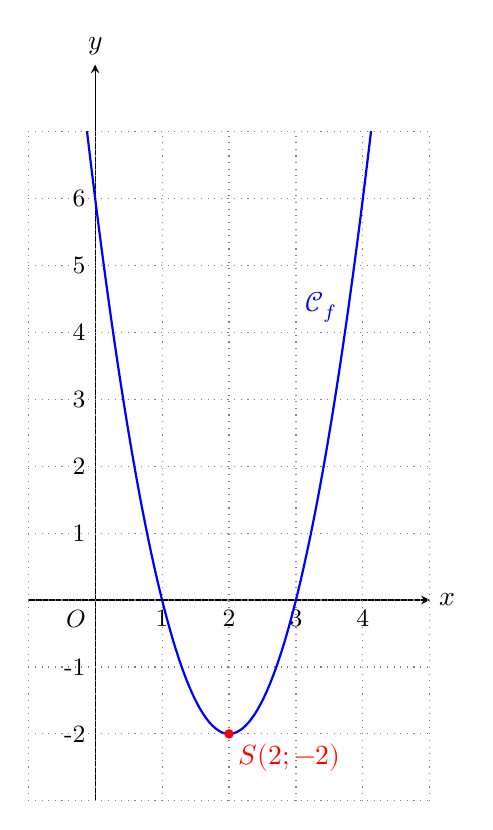
\begin{tikzpicture}[scale=0.85]
  \draw[->, >=stealth] (-1,0) -- (5,0) node[right] {$x$};
  \draw[->, >=stealth] (0,-3) -- (0,8) node[above] {$y$};
  \draw[dotted, gray] (-1,-3) grid (5,7);
  \foreach \x in {1,2,3,4}
    \draw (\x,0) node[below, font=\small] {\x};
  \foreach \y in {-2,-1,1,2,3,4,5,6}
    \draw (0,\y) node[left, font=\small] {\y};
  \draw (0,0) node[below left, font=\small] {$O$};
  \begin{scope}\clip (-1.0,-3.0) rectangle (5.0,7.0);
  \draw[thick, blue, domain=-0.25:4.25, samples=100] plot (\x, {2*(\x)^2 - 8*\x + 6});
  \end{scope}
  \node[blue, above right] at (3,4) {$\mathcal{C}_f$};
  \fill[red] (2,-2) circle (2pt) node[below right] {$S(2;-2)$};
\end{tikzpicture}
\end{center}

\newpage

% ==================== SUJET B (ÉLÈVE ANTI-TRICHE) ====================
\sujet{B}

\exo{1}{Forme canonique, factorisation et lecture graphique (Variante)}
Soit $g$ la fonction définie sur $\mathbb{R}$ par $g(x) = 2x^2 + 8x + 6$.  
On note $\mathcal{C}_g$ sa courbe représentative dans un repère orthogonal $(O, \vec{i}, \vec{j})$.

\begin{enumerate}
  \item \textbf{Forme canonique :}
  \begin{enumerate}
    \item Montrer que pour tout réel $x$, $g(x) = 2(x + 2)^2 - 2$.
    \item En déduire les coordonnées du sommet $S'$ de la parabole $\mathcal{C}_g$ ainsi que son sens de variation.
  \end{enumerate}
  \item \textbf{Factorisation et racines :}
  \begin{enumerate}
    \item Vérifier que $-1$ est une racine évidente de $g(x)$. En déduire la factorisation de $g(x)$ sous la forme $g(x) = 2(x + 1)(x - x_2')$ où $x_2'$ est à déterminer.
    \item Résoudre dans $\mathbb{R}$ l'équation $g(x) = 0$.
  \end{enumerate}
  \item \textbf{Exploitation graphique :}
  \begin{enumerate}
    \item Préciser l'ordonnée du point d'intersection de $\mathcal{C}_g$ avec l'axe des ordonnées.
    \item Par lecture graphique ou par le calcul, déterminer les coordonnées des points d'intersection de $\mathcal{C}_g$ avec l'axe des abscisses.
  \end{enumerate}
\end{enumerate}

\begin{center}
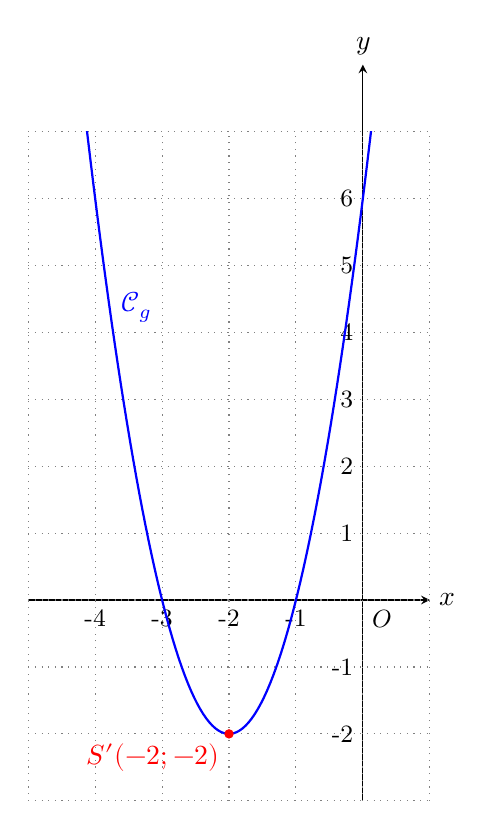
\begin{tikzpicture}[scale=0.85]
  \draw[->, >=stealth] (-5,0) -- (1,0) node[right] {$x$};
  \draw[->, >=stealth] (0,-3) -- (0,8) node[above] {$y$};
  \draw[dotted, gray] (-5,-3) grid (1,7);
  \foreach \x in {-4,-3,-2,-1}
    \draw (\x,0) node[below, font=\small] {\x};
  \foreach \y in {-2,-1,1,2,3,4,5,6}
    \draw (0,\y) node[left, font=\small] {\y};
  \draw (0,0) node[below right, font=\small] {$O$};
  \begin{scope}\clip (-5.0,-3.0) rectangle (1.0,7.0);
  \draw[thick, blue, domain=-4.25:0.25, samples=100] plot (\x, {2*(\x)^2 + 8*\x + 6});
  \end{scope}
  \node[blue, above left] at (-3,4) {$\mathcal{C}_g$};
  \fill[red] (-2,-2) circle (2pt) node[below left] {$S'(-2;-2)$};
\end{tikzpicture}
\end{center}

\newpage

% ==================== CORRIGÉS DÉTAILLÉS ====================
\begin{center}
  {\LARGE \textbf{CORRIGÉ OFFICIEL \& BARÈME}}\\[0.4em]
  {\large Sujet A et Sujet B}
\end{center}

\partie{Corrigé du Sujet A (Barème sur 10 points)}
\begin{enumerate}
  \item \textbf{Forme canonique (3 pts) :}
  \begin{enumerate}
    \item Développement : $2(x - 2)^2 - 2 = 2(x^2 - 4x + 4) - 2 = 2x^2 - 8x + 8 - 2 = 2x^2 - 8x + 6 = f(x)$. \emph{(1,5 pt)}
    \item Sommet $S(2 ; -2)$. Comme $a = 2 > 0$, la parabole est décroissante puis croissante. \emph{(1,5 pt)}
  \end{enumerate}
  \item \textbf{Factorisation et racines (4 pts) :}
  \begin{enumerate}
    \item $f(1) = 2(1)^2 - 8(1) + 6 = 0$. $1$ est racine. On trouve $f(x) = 2(x - 1)(x - 3)$. \emph{(2 pts)}
    \item $f(x) = 0 \iff x = 1$ ou $x = 3$. \emph{(2 pts)}
  \end{enumerate}
  \item \textbf{Exploitation graphique (3 pts) :}
  \begin{enumerate}
    \item Ordonnée à l'origine : $f(0) = 6$ (point $(0 ; 6)$). \emph{(1 pt)}
    \item Intersections avec l'axe des abscisses : $(1 ; 0)$ et $(3 ; 0)$. \emph{(2 pts)}
  \end{enumerate}
\end{enumerate}

\vspace{1.5em}
\partie{Corrigé du Sujet B (Barème sur 10 points)}
\begin{enumerate}
  \item \textbf{Forme canonique (3 pts) :}
  \begin{enumerate}
    \item Développement : $2(x + 2)^2 - 2 = 2(x^2 + 4x + 4) - 2 = 2x^2 + 8x + 8 - 2 = 2x^2 + 8x + 6 = g(x)$. \emph{(1,5 pt)}
    \item Sommet $S'(-2 ; -2)$. Parabole décroissante puis croissante ($a = 2 > 0$). \emph{(1,5 pt)}
  \end{enumerate}
  \item \textbf{Factorisation et racines (4 pts) :}
  \begin{enumerate}
    \item $g(-1) = 2(-1)^2 + 8(-1) + 6 = 0$. $-1$ est racine. On trouve $g(x) = 2(x + 1)(x + 3)$. \emph{(2 pts)}
    \item $g(x) = 0 \iff x = -3$ ou $x = -1$. \emph{(2 pts)}
  \end{enumerate}
  \item \textbf{Exploitation graphique (3 pts) :}
  \begin{enumerate}
    \item Ordonnée à l'origine : $g(0) = 6$ (point $(0 ; 6)$). \emph{(1 pt)}
    \item Intersections avec l'axe des abscisses : $(-3 ; 0)$ et $(-1 ; 0)$. \emph{(2 pts)}
  \end{enumerate}
\end{enumerate}

\end{document}
